\chapter{Obiettivi}
In un mondo sempre più interconnesso e in rapida evoluzione, approcci statici al machine learning possono diventare impraticabili quando si tratta di produrre sistemi in grado di adattarsi dinamicamente allo stato fisico e mentale degli utenti che vi interagiscono. Inoltre, con l'ampia presenza di dispositivi in grado di raccogliere anche in tempo reale informazioni sulla condizione attuale degli utenti, diventano continuamente disponibili nuovi dati con cui perfezionare i modelli di machine learning in uso attraverso tecniche di continual learning.
\section{Stato dell'Arte}
\subsection{Continual Learning} L'ambito del continual learning è in continua evoluzione. Negli ultimi anni, studi come \textit{Learning without Forgetting}$^{\cite{li2017learning}}$ o \textit{Overcoming catastrophic forgetting in neural networks}$^{\cite{kirkpatrick2017overcoming}}$ hanno affrontato il problema del \textit{catastrophic forgetting} proponendo soluzioni da adottare durante l'addestramento delle reti neurali. In \textit{Learning without Forgetting} viene proposto l'omonimo approccio, LWF, che non usa dati relativi alla conoscenza già appresa ma solo i nuovi dati relativi alla nuova conoscenza, imparando parametri del modello specifici per i nuovi dati ma che abbiano performance non impattatti sulla conoscenza già presente. Nel secondo studio viene proposto un algoritmo che prende il nome di \textit{Elastic Weight Consolidation}, o EWC, che interpreta i parametri da apprendere della rete neurale come spazi probabilistici, e rende meno probabile la modifica di quei parametri che risultano importanti per la conoscenza già appresa quando si addestra su nuova conoscenza.\\
Ulteriori studi hanno proposto approcci definiti \textit{reharsal} o di replay$^{\cite{DBLP:journals/corr/Lopez-PazR17},\cite{rolnick2019experience}}$. Queste tecniche consistono nel mantenere in memoria, all'interno di buffer, degli esempi della conoscenza passata selezionati secondo qualche politica. Durante le fasi di addestramento successive, ai nuovi dati vengono intervallati gli esempi mantenuti in memoria, così da consentire al modello di "ricordare" la conoscenza passata e mantenerla, mitigando così il \textit{catastrophic forgetting}.\\\\
Altre ricerche hanno proposto metriche per misurare le performance dell'apprendimento continual e l'impatto che questo approccio ha sulla vecchia e nuova conoscenza, come in \textit{Gradient Episodic Memory for Continual Learning}$^{\cite{DBLP:journals/corr/Lopez-PazR17}}$ dove vengono proposte metriche per misurare il \textit{forward transfer}, FWT, e il \textit{backward transfer}, BWT: con queste due metriche si misura l'impatto che la nuova conoscenza ha sulla conoscenza, rispettivamente, già appresa e su quella che si andrà ad apprendere.\\\\
Altri recenti studi nell'ambito del continual learning si sono concentrati, ad esempio, sull'applicabilità pratica e l'ideazione di un'architettura in grado di manutenere modelli di machine learning in produzione e gestire la dinamicità e i cambiamenti sui dati$^{\cite{diethe2019continual}}$, oppure in ambiti come la \textit{human activity recognition} (HAR)$^{\cite{Jha_2021}}$, cioè il riconoscimento delle attività quotidiane delle persone attraverso dei sensori, o ancora l'acquisizione di informazioni dai social media per, ad esempio, gestire al meglio situazioni di crisi$^{\cite{priyanshu2021continual}}$.\\
In tutti questi ambiti il continual learning si rivela fondamentale per adattare dinamicamente i modelli di machine learning al mutevole ambiente reale, senza la necessità di addestrare continuamente nuovi modelli da zero con l'ulteriore difficoltà costituita dal memorizzare dati anche molto vecchi portando a dataset di dimensioni elevate che aumentano il tempo necessario all'addestramento. Grazie al continual learning, invece, possiamo mantenere solo una parte (negli approcci cosiddetti di \textit{reharsal} o \textit{replay}) o non mantenere affatto esempi relativi alla conoscenza precedente.\\\\
In molti studi, l'approccio al continual learning è stato suddiviso in tre scenari fondamentali$^{\cite{vandeven2019generative},\cite{vandeven2019scenarios}}$. Viene presa in considerazione una rete neurale che deve apprendere in maniera sequenziale una serie di task, dove con task si indica una qualsiasi attività che la rete neurale deve svolgere (ad esempio, classificare le razze dei cani che appaiono in un immagine):
\begin{itemize}
    \item[-] \textbf{Task-IL}, o \textit{task incremental}: viene indicato il task a cui appartiene il problema, tra i task già appresi dal modello, e viene chiesto di risolverlo
    \item[-] \textbf{Domain-IL}, o \textit{domain incremental}: viene chiesto di risolvere il problema senza indicare il task a cui appartiene tra quelli appresi
    \item[-] \textbf{Class-IL}, o \textit{class incremental}: viene chiesto di risolvere il problema e anche di identificare a quale task esso appartiene
\end{itemize}
Un dataset molto usato nell'ambito del machine learning è il MNIST, un database di cifre manoscritte che viene usato per valutare modelli, approcci e algoritmi riguardanti l'addestramento e il comportamento dei modelli di classificazione delle immagini (Figura \ref{fig:mnistexamples}).
\begin{figure}[h]
	\begin{center}
		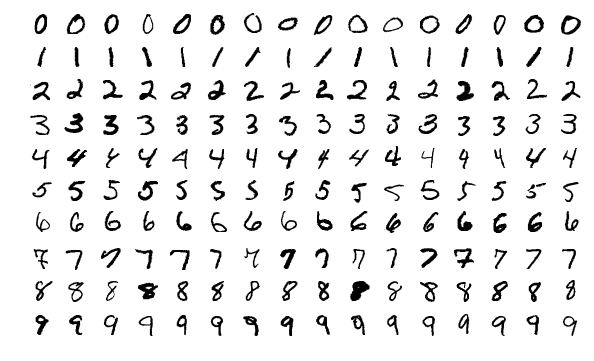
\includegraphics[width=0.75\textwidth]{img/MnistExamples.png}
		\caption{Esempio dei dati del MNIST}
		\label{fig:mnistexamples}
	\end{center}
\end{figure}
Per meglio comprendere i tre scenari proposti, i task relativi al dataset MNIST possono essere individuati nei seguenti:
\begin{itemize}
    \item[-] Task 1: identificare tra 0 e 1
    \item[-] Task 2: identificare tra 2 e 3
    \item[-] Task 3: identificare tra 4 e 5
    \item[-] Task 4: identificare tra 6 e 7
    \item[-] Task 5: identificare tra 8 e 9
\end{itemize}
Con questi task, i tre scenari individuati diventano:
\begin{itemize}
    \item[-] \textbf{Task-IL}: dato il task, è la prima o la seconda classe? Ad esempio, identificare fra 0 e 1
    \item[-] \textbf{Domain-IL}: senza sapere il task, è la prima o la seconda classe? Ad esempio, identificare se è un numero pari (prima classe) o dispari (seconda classe)
    \item[-] \textbf{Class-IL}: senza sapere il task, che cifra è? Nell'esempio, individuare quale cifra è da 0 a 9
\end{itemize}
\subsection{Reti Neurali Ricorrenti}
Una rete neurale ricorrente, o RNN, è una rete neurale dove i neuroni, o alcuni di essi, sono collegati a sé stessi in un ciclo chiuso. Questo collegamento consente ai layer di una RNN di mantenere informazioni in maniera analoga ad uno stato interno, permettendo di modellare, ad esempio, i comportamenti dinamici di una sequenza temporale fornita come input, dove ogni dato dipende anche dai dati precedenti già ricevuti.\\
In letteratura esistono diverse architetture di reti neurali ricorrenti, ma molte di esse devono la loro esistenza a due nodi ricorrenti fondamentali: le \textit{Long Short-Term Memory}, LSTM, e le \textit{Gated Recurrent Unit}, GRU (Figura \ref{fig:rnnlstmgru}). 
\begin{figure}[h]
	\begin{center}
		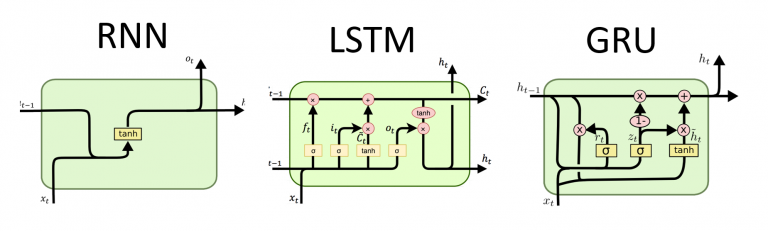
\includegraphics[width=0.95\textwidth]{img/rnnlstmgru.png}
		\caption{Schemi di nodi ricorrenti}
		\label{fig:rnnlstmgru}
	\end{center}
\end{figure}
LSTM e GRU hanno meccanismi interni, chiamati \textit{gates} o cancelli, che regolano il flusso delle informazioni. Attraverso questi \textit{gate}, le unità apprendono quali dati sono importanti all'interno della sequenza e quali si possono ignorare, lasciando così al resto della rete solamente le informazioni che ritiene essere rilevanti per fare predizioni.\\\\
In una LSTM, i dati passano attraverso il \textit{forget gate}, che decide immediatamente quali informazioni è utile mantenere e quali ignorare. Dopodiché i dati passano attraverso l'\textit{input gate} assieme allo stato precedente dell'unità, che decide quali valori dello stato interno conviene aggiornare, e queste informazioni sono poi usate per aggiornare lo stato dell'unità. Infine, attraverso l'\textit{output gate} viene calcolato il nuovo stato interno dell'unità, che servirà all'input successivo.\\\\
Nelle GRU abbiamo un comportamento simile, ma la struttura dell'unità è semplificata. I dati passano subito attraverso il \textit{update gate}, che si comporta in modo simile ai \textit{gate} \textit{forget} e \textit{input} dell'LSTM, decidendo quali informazioni ignorare e quali mantenere. Dopodiché si attraversa il \textit{reset gate}, che decide cosa mantenere delle informazioni precedententemente analizzate. Avendo una struttura più semplificata, la GRU sono solitamente più veloci delle LSTM.
\pagebreak
\subsection{Software e hardware}
Negli ultimi anni sono nate diverse librerie software che consentono di realizzare modelli di machine learning performanti in breve tempo dei tipi più disparati, da semplici modelli lineari a reti neurali profonde convolutive e oltre.\\
Librerie open source come PyTorch, Tensorflow$^{\cite{abadi2016tensorflow}}$ e Keras, ma anche librerie proprietarie come Apple Core ML, IBM Watson e MATLAB Deep Learning Toolbox, hanno aperto le porte del machine learning a chiunque sia disposto a studiarle. Alcune librerie, come in particolare TensorFlow 2.0, possiedono API estremamente semplici che consentono di eseguire il preprocessing dei dataset, strutturare una rete neurale, addestrarla e valutarla con una manciata di righe di codice, e nonostante la semplicità essa consente comunque di mettere mano e andare a personalizzare ogni minimo aspetto di tutte le fasi, dal preprocessing al training. In letteratura sono disponibili anche moltissimi testi che consentono di approcciarsi facilmente al machine learning$^{\cite{chollet},\cite{geron}}$.\\\\
Anche a livello hardware gli ultimi anni hanno portato enormi sviluppi, grazie soprattutto all'industria videoludica e alle criptovalute che hanno spinto la ricerca e lo sviluppo di processori specializzati in calcolo parallelo e matriciale. Questi dispositivi, denominati \textit{Graphics Processing Unit} o GPU, consentono di ridurre esponenzialmente i tempi di addestramento delle reti neurali, abbassando ancora di più i requisiti per accedere a questo campo di studi e consentendo l'esecuzione di modelli di machine learning anche su un comune computer casalingo.\\
Inoltre, aziende come Google hanno sviluppato hardware realizzato ad hoc per le computazioni necessarie alle reti neurali, incrementando così ulteriormente la velocità e l'efficienza di questi modelli. Nel caso di Google, questo hardware è chiamato \textit{Tensor Processing Unit} o TPU.

\section{Scopo del lavoro}  % ugly title
\subsection{Applicazioni future}
Alla luce degli attuali studi nell'ampio campo che è il machine learning, e in particolare riguardanti il continual learning e lo HSM, diventa chiaro come il futuro richiederà sempre più responsività ai sistemi predittivi e un sempre maggior grado di adattamento allo stato psico-fisico del momento dell'utente. Questa necessità di continua evoluzione ben si sposa con le caratteristiche del continual learning, e possibili applicazioni di questa sinergia continual learning -- HSM si possono individuare in diversi contesti, tra cui ad esempio:
\pagebreak
\begin{itemize}
    \item[-] \textbf{Guida autonoma}.\\La crescente industria dei veicoli a guida autonoma ha portato ad uno sviluppo in moltissimi campi del machine learning$^{\cite{huang2020autonomous}}$, in particolare nel campo dell'\textit{object recognition}$^{\cite{Carranza_Garc_a_2021}}$, del \textit{behavioral planning}$^{\cite{6856582}}$ e altri ancora. L'\textit{autonomous driving} negli ultimi anni è, senza dubbio, uno dei motori principali nello sviluppo della disciplina del machine learning.\\
    Un veicolo a guida autonoma che sappia adattarsi allo stato psico-fisico attuale del conducente può portare a grossi benefici: ad esempio, essere in grado di modificare il proprio andamento per accomodare uno stato di malessere mitigando così il rischio di incidenti, o poter proporre tappe durante il percorso a seconda della condizione dei passeggeri portando così a più piacevole utilizzo del sistema da parte degli utenti.
    \item[-] \textbf{Intrattenimento}.\\L'industria dell'intrattenimento si è sempre interessata alle nuove tecnologie, puntando alla novità del momento in modo da raggiungere un pubblico sempre più ampio: ad esempio, la tecnologia degli schermi 3D o della realtà virtuale.\\
    Un sistema adattivo di riconoscimento dello stato psico-fisico dello spettatore o del videogiocatore può portare a esperienze multimediali più realistici e responsivi, che ad esempio possano adattare la propria narrazione o l'atmosfera proposta all'utente in maniera da sfruttare, o alleviare, eventuali emozioni che nascono nello spettatore.
    \item[-] % TODO altri esempi: interfacce che si modulano in base allo stato mentale del momento?
\end{itemize}
Tutti questi ambiti, per poter avere risultati ottimi, devono essere in grado di adattarsi e specializzarsi nel riconoscere lo stato psico-fisico del singolo utente: il conducente proprietario del veicolo, il videogiocatore che possiede la console\ldots ottenendo così sistemi calibrati e personalizzati in base alle caratteristiche e alle esigenze del singolo utente.\\\\
Questa sinergia risulta ancora poco studiata in letteratura, quindi può essere utile mettere sotto esame alcune tecniche di continual learning attualmente studiate per giudicare la loro applicabilità o meno in contesti di \textit{human state monitoring}, così da concludere se siano necessari ulteriori sforzi in questa direzione per poter realizzare, in futuro, sistemi sempre più integrati con l'uomo e interfacce uomo-macchina sempre più intuitive e adattive. Valutare fin da subito l'applicabilità di questa sinergia è fondamentale in un campo di studi che si muove così in fretta come quello del machine learning.
\pagebreak
\subsection{Obiettivi} % \/ ricerca? studio?
Gli obiettivi di questo progetto sono i seguenti:
\begin{itemize}
    \item[-] \textbf{Individuare dataset contenenti dati realitivi allo \textit{human state monitoring}}\\
    Per poter valutare la sinergia tra continual learning e \textit{human state monitoring}, inanzitutto si rende necessaria la raccolta di dati riguardanti lo HSM. Ne sono stati individuati due, scelti per le caratteristiche che verranno discusse in seguito: WESAD$^{\cite{10.1145/3242969.3242985}}$ e ASCERTAIN$^{\cite{7736040}}$.
    \item[-] \textbf{Selezionare le metriche e le informazioni utili alla comparazione dei vari approcci}\\
    Comparare i vari approcci significa avere a disposizione per ognuno di essi delle metriche che vadano a misurare i loro vari aspetti, come il tempo necessario all'addestramento, l'accuratezza raggiunta, la conoscenza trasferita e l'impatto a livello di memoria.
    \item[-] \textbf{Scegliere una \textit{baseline}}\\
    Cioè un approccio base da cui partire e che sia utile a confrontare tutti gli altri. Come sarà specificato in seguito, l'approccio scelto come baseline sarà quello \textit{offline}: ciò consiste nell'addestramento di una rete neurale usando l'intero training set a disposizione senza usare approcci continual.
    \item[-] \textbf{Raccogliere i dati necessari}\\
    Si rende necessario individuare un ambiente su cui poter eseguire le computazioni necessarie all'addestramento, trovare le API e i linguaggi di programmazione adatti allo scopo e produrre del codice verificabile e degli esperimenti replicabili.
    \item[-] \textbf{Confrontare i risultati e trarre le conclusioni}\\
    Una volta raccolti tutti i dati necessari, essi verranno confrontati per poter finalmente valutare la sinergia fra continual learning e human state monitoring.
\end{itemize}
